\newpage
%\pagestyle{empty}

\begin{minipage}[c]{.25\linewidth}
	
\includegraphics[width=4cm]{images/LEnsE_IOGS.jpg}
\end{minipage} \hfill
\begin{minipage}[c]{.4\linewidth}

\begin{center}
\vspace{0.3cm}
{\Large \textsc{Opto-Électronique}}

\medskip

5N-027-SCI \qquad \textbf{\Large TD Séance 3}

\end{center}
\end{minipage}\hfill

%%%%%%%%%%%%%%%%%%%%%%%%%%%%%%%%%%
\section{TD3 - Diodes}


%%%%%%%%%%%%%%%%%%%%%%%%%%%%%%%%%%%%%%%%%%%%%%%%%%%%%%%
\subsection{Exercice 0 - Caractéristique d'une diode}

\begin{enumerate}
	\item Rappeler la caractéristique statique d'une diode.
	\item Dans le cas d'une LED, dans quelle partie de la caractéristique émet-elle des photons ?
	\item Dans le cas d'une photodiode, dans quelle partie de la caractéristique peut-elle servir de capteur de photons ?
\end{enumerate}


%%%%%%%%%%%%%%%%%%%%%%%%%%%%%%%%%%%%%%%%%%%%%%%%%%%%%%%
\subsection{Exercice 1 - Émettre des photons à partir d'une LED}

On souhaite réaliser un montage émetteur à l'aide d'une \textbf{diode rouge} de type KingBright L-53HD. On propose d'étudier le montage suivant :

\begin{center}
	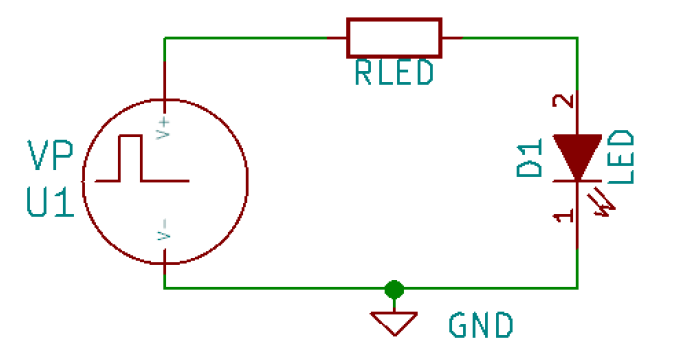
\includegraphics[width=5cm]{images/emetteur_003_a.png}
\end{center}

On donne une partie de la documentation : 

\begin{center}
	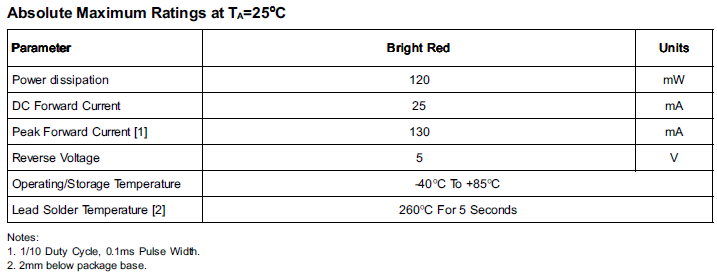
\includegraphics[width=14cm]{images/doc_led_rouge.png}
\end{center}

\begin{enumerate}
	\item Cas 1 : La source de tension $V_P$ est une \textbf{source continue}. Elle délivre une différence de potentiel de $5\operatorname{V}$.
	\begin{enumerate}
		\item Quelle est la valeur maximale du courant que la diode peut supporter dans ces conditions ?
		\item Quelle est la valeur minimale que doit avoir $R_{LED}$ pour respecter cette condition ?
		\item Quel sera alors le courant moyen qui traversera la LED ?
	\end{enumerate}
	
	\item Cas 2 : La source de tension $V_P$ est une \textbf{source impulsionnelle}. Elle délivre des impulsions de $5\operatorname{V}$ de durée $0.1\operatorname{ms}$ avec une fréquence de répétition de $1\operatorname{kHz}$.
	\begin{enumerate}
		\item Quelle est la valeur maximale du courant que la diode peut supporter dans ces conditions ?
		\item Quelle est la valeur minimale que doit avoir $R_{LED}$ pour respecter cette condition ?
		\item Quel sera alors le courant moyen qui traversera la LED ?
	\end{enumerate}
\end{enumerate}


%%%%%%%%%%%%%%%%%%%%%%%%%%%%%%%%%%%%%%%%%%%%%%%%%%%%%%%
\subsection{Exercice 2 - Modifier la forme d'une tension}{

On considère les deux montages suivants :

\begin{center}
	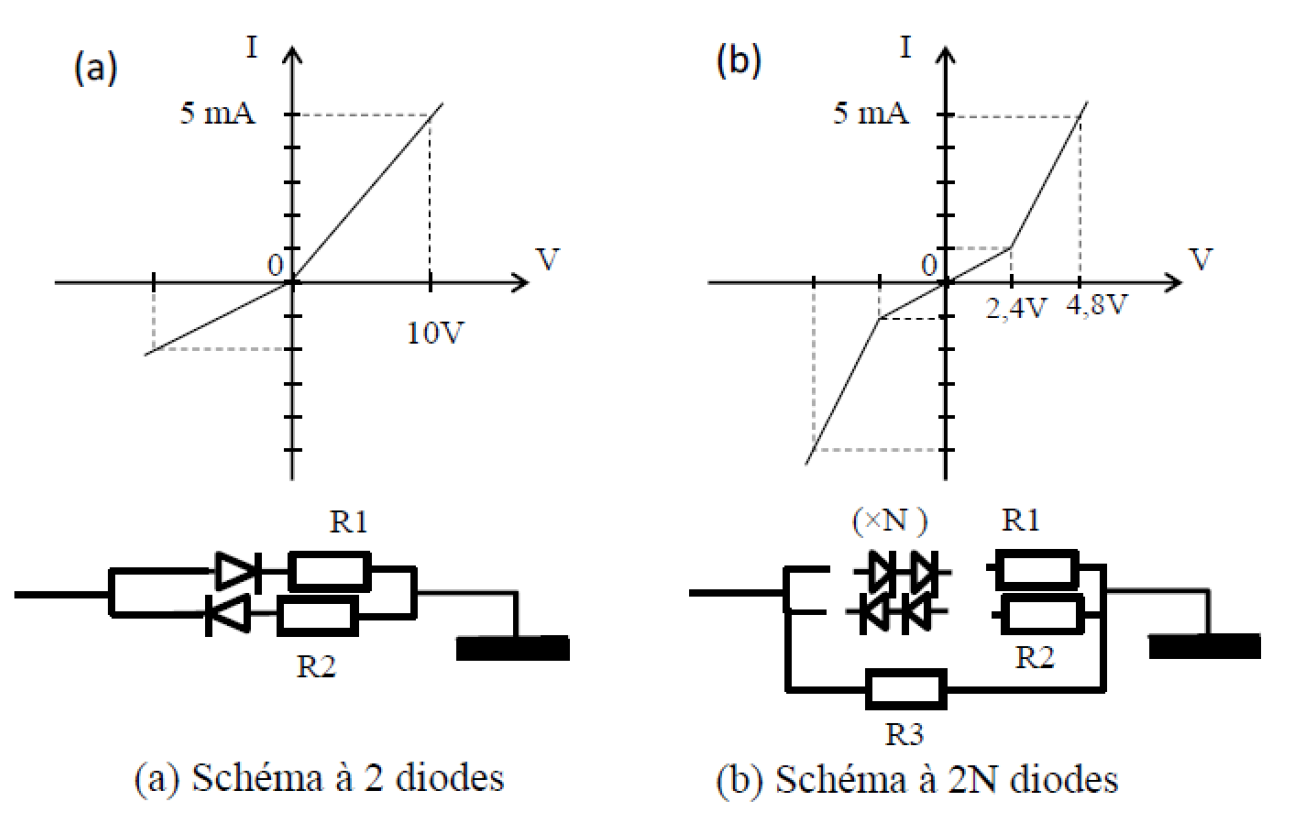
\includegraphics[width=12cm]{images/diodes_002_a.png}
\end{center}

\begin{enumerate}
	\item Dans le cas du montage de la figure (a) et d'utilisation de diodes parfaites et idéales, que doivent valoir $R_1$ et $R_2$ pour obtenir la caractéristique tracée dans le graphe $I(V)$ ?
	\item Dans le cas du montage de la figure (b), les diodes ont pour seuil $0,6\operatorname{V}$. Que doivent valoir $R_1$, $R_2$ et $R_3$ et le nombre de diodes $N$ ($N = 2$ a été dessiné arbitrairement) pour obtenir la caractéristique tracée dans le graphe $I(V)$ ?
\end{enumerate}


%%%%%%%%%%%%%%%%%%%%%%%%%%%%%%%%%%%%%%%%%%%%%%%%%%%%%%%
\subsection{Exercice 3 - Limiter une tension}

Soit le circuit suivant :

\begin{center}
\begin{circuitikz}
	\draw (0,0) to[battery2, invert] (0,5) to[short, -] (6,5)
		to[full diode=$D_1$, invert, i<_=$i_1$	] (6,2.5) to[full diode=$D_2$, invert, i<_=$i_2$, *-] (6,0)
		to[short, -*] (3,0) node[ground](GND){} to[short, -] (0,0);
	\draw (3,0) to[sV] (3,2.5) to[R=$R_p$, i=$i_R$] (6,2.5);
	\draw (6,2.5) to[short, -o] (8,2.5);
	\draw (8, 0) to[short, -o] ++(0,0) node[ground](GND){};
	\draw (8,0.3) edge[->,color={red}] (8, 2.2);
	\node[text={red}] (Vs) at (8.5,1.3){$V_S$}; 
	\draw (7,0.3) edge[<-,color={blue}] (7, 2.2);
	\node[text={blue}] (Vd2) at (7.5,1.3){$V_{D2}$}; 
	\draw (7,4.7) edge[->,color={blue}] (7, 2.8);
	\node[text={blue}] (Vd1) at (7.5,3.7){$V_{D1}$}; 
	\draw (2.5,0.3) edge[->,color={green!40!black}] (2.5, 2.2);
	\node[text={green!40!black}] (Ve) at (2,1.3){$V_e$}; 
	\draw (0.7,0.3) edge[->,color={black}] (0.7, 4.7);
	\node[text={black}] (Vcc) at (1.3, 2.5){$V_{CC}$}; 
\end{circuitikz}
\end{center}


\begin{enumerate}
	\item Sous quelles conditions sur $V_S$ la diode $D_1$ est-elle passante ? De même pour la diode $D_2$ ?
	\item Donnez la forme du signal de sortie $V_S$ si on suppose que le signal $V_e$ est sinusoIdal d'amplitude $2 \cdot V_{CC}$ et de valeur moyenne nulle.
\end{enumerate}


%%%%%%%%%%%%%%%%%%%%%%%%%%%%%%%%%%%%%%%%%%%%%%%%%%%%%%%